\documentclass[12 pt, a4paper]{article}
\usepackage[norsk]{babel}  								% For norsk oppsett
\usepackage[utf8]{inputenc}
\usepackage{amsmath}
\usepackage{amssymb}
\usepackage{graphicx}
\usepackage{subcaption}
\usepackage{hyperref}
\usepackage{fancyhdr}
\usepackage{enumerate}
\usepackage{float}
\usepackage{tikz}
\usepackage{circuitikz}
\usepackage{tabularx}
\usepackage{physics}
%\usepackage[includeheadfoot, margin =1cm]{geometry}
%\usepackage{python}
\usepackage[version=3]{mhchem}
\usepackage{siunitx}
\usepackage{todonotes}
\usepackage{xcolor}
\usepackage{lastpage}
\usepackage{listings}
\renewcommand{\exp}[1]{\mathrm{e}^{#1}}

\lstset{basicstyle=\ttfamily,
  showstringspaces=false,
  commentstyle=\color{red},
  keywordstyle=\color{blue}
}

\usepackage[bottom]{footmisc}
\renewcommand\footnoterule{\rule{\linewidth}{0.5pt}}

\setlength{\parindent}{0cm}

\author{Mikael B. Kiste}
\title{STK1000 - oblig 1}

\begin{document}
\maketitle
\newpage

%\pagestyle{fancy}
%\fancyhf{}
%\rhead{STK1000 - Oblig 1}
%\lhead{Erik Skaar}
%\fancyfoot[CE,LO]{\leftmark}
%\fancyfoot[LE,RO]{Page \number\value{page} of \pageref{LastPage}}

%\renewcommand{\headrulewidth}{2pt}
%\renewcommand{\footrulewidth}{1pt}

\section{}%1

\subsection*{a}
Her er et histogram av BMR verdiene til sebrafinkene. Histogrammet ser normalfordelt ut, med en god del sebrafinker som har en BMR verdi nær gjennomsnittet og et kraftig avtagende antall finker jo lenger man går vekk fra gjennomsnittet. 
\begin{figure}[H]
		\centering
		\includegraphics[width=0.9\linewidth]{zebrafish.pdf}
		\caption{Histogram av BMR-verdiene til 150 zebrafisker}
		\label{fig:histogram}
\end{figure}


\subsection*{b}

Ved å bruke kommandoen \texttt{mean} i R får jeg gjennomsnitt og \texttt{median} gir meg median.
\begin{align*}
    \bar{x} = 0.8485003\mathrm{mL}\frac{o_2}{\mathrm{m}}\\
    \mathrm{mean} = 0.8397846\mathrm{mL}\frac{o_2}{\mathrm{m}}
\end{align*}
Gjennomsnittet tar summen av måleverdien til alle datapunktene før det deler på antall datapunkter mens median er verdien på det midterste elementet i en ordnet (numerisk økende) liste av datapunktene.

\subsection*{c}

Ved å bruke kommandoen \texttt{IQR} i R får jeg inter-kvartil og \texttt{sd} gir meg standardavvik.
\begin{align*}
    \mathrm{IQR} = 0.1517731\mathrm{mL}\frac{o_2}{\mathrm{m}}\\
    \sigma = 0.1134001\mathrm{mL}\frac{o_2}{\mathrm{m}}
\end{align*}

\subsection*{d}

Ved å bruke kommandoene \texttt{qqnorm()} i R får jeg inter-kvartil og \texttt{sd()} gir meg standardavvik.

\begin{figure}[H]
		\centering
		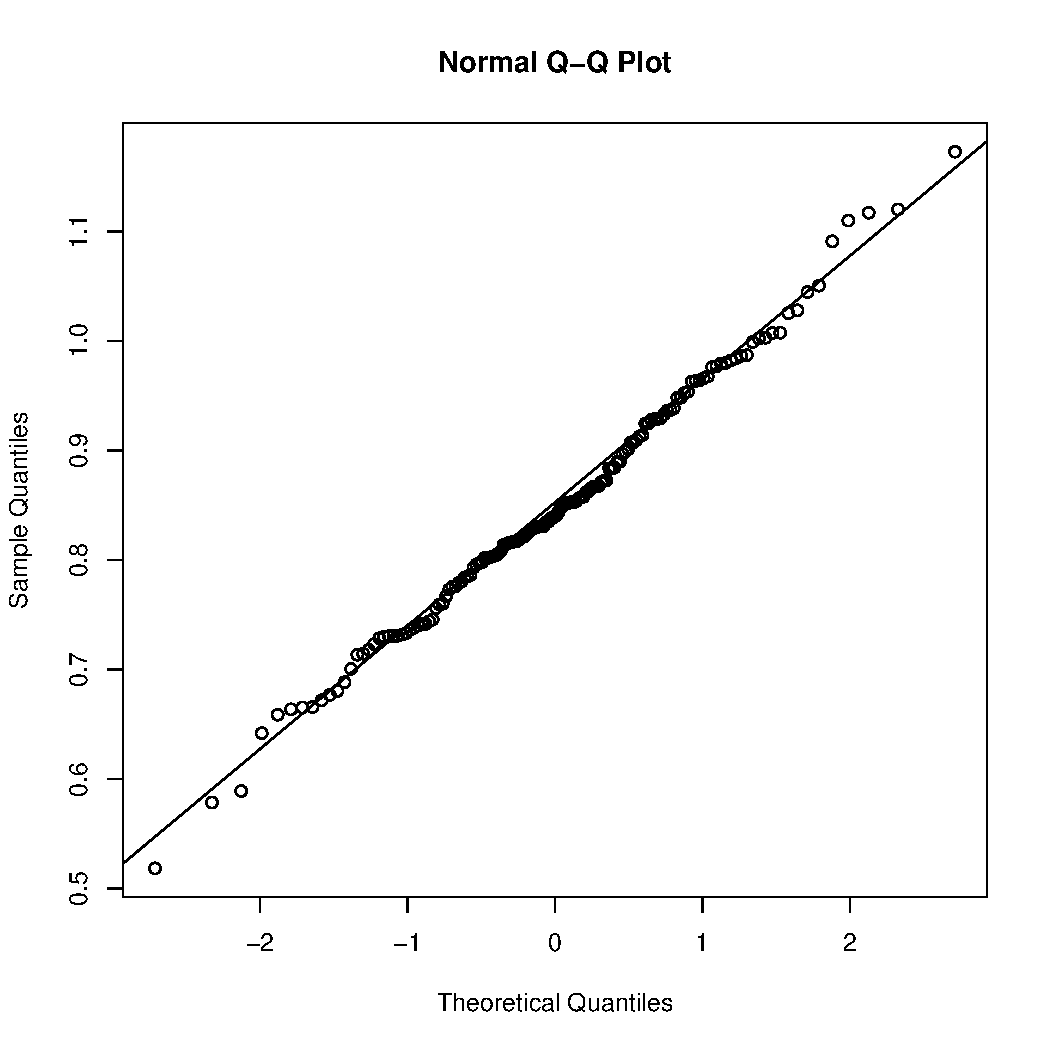
\includegraphics[width=0.9\linewidth]{Rplots.pdf}
		\caption{Figuren viser målte verdier mot standardavviket vi fikk tidligere i oppgaven}
		\label{fig:QQ}
\end{figure}
Plottet indikerer hvordan de målte verdiene har fordelt seg i forhold til standardavviket. Igjen ser man at de fleste datapunktene legger seg rundt gjennomsnittet, men i tillegg får man et inntrykk av hvordan målverdiene avviker fra den teoretiske perfekte normalfordelingen (over eller under den lineære funksjonen). Man kan se at dataen passer ganske bra til en normalfordeling.

\subsection*{e}

Standardiserte verdien til BMR:
Den standardiserte verdien, eller 'z-score', antyder hvor mange standardavvik en målverdi er fra gjennomsnittet. Altså

\begin{align*}
    z = \frac{x - \mu}{\sigma}
\end{align*}

For BMR = 0.8 mL O$_2$/min gir det:
\begin{align*}
    z = \frac{x - \mu}{\sigma} = \frac{0.8 - 0.8485003}{0.1134001} \approx -0.43
\end{align*}
Målverdien på $0.8\mathrm{mL}\frac{o_2}{\mathrm{m}}$ er $-0.43$ standardavvik unna gjennomsnittet.

\subsection*{f}

Ved å bruke kommandoen \texttt{pnorm()} i R får jeg prosentilen til en BMR på $0.6$
\begin{align*}
    p(x<0.6) = 0.01421294
\end{align*}

\subsection*{g}
På samme måte som i forrige oppgave bruker jeg \texttt{pnorm()}, men denne gangen tar jeg én og trekker i fra sannsynligheten for å finne ut sannsynligheten for at en fink har en BMR som er OVER dette.)
\begin{align*}
    p(x>1.0) = 0.09077876
\end{align*}

\pagebreak
\section{}


\subsection*{a}
Kvantitative variabler er variabler som har en konkret tallverdi. Dette tillater at flere nyttige numeriske operasjoner kan utføres på et datasett av kvantitative variabler. Konsentrasjon av kortisol og testosteron er også kvantitative\\
Kvalitative variabler derimot kan være mer abstrakte. Som for eksempel øyenfarge.\\
Kategoriske variabler er alltid medlemmer av et gitt sett av mulige verdier. Innen vitenskap er det for eksempel fortsatt slik at nesten utelukkende alle dyr kun kan ha ett av to kjønn: han (maskulin) eller hun (feminin). Kjønn er altså et eksempel på en kategorisk variabel. I dette tilfellet er også populasjon kategorisk når den kun deler populasjonen inn i ulv som er hardt jaktet eller ikke. Legg merke til at denne også er en kvalitativ variabel. Kategoriske variabler kan være enten kvalitative eller kvantitative.

\subsection*{b}

Ved å bruke kommandoene \texttt{pie(table(variabel))} i R får jeg et kakediagram over de kategoriske variablene. 

\begin{figure}[H]
		\centering
		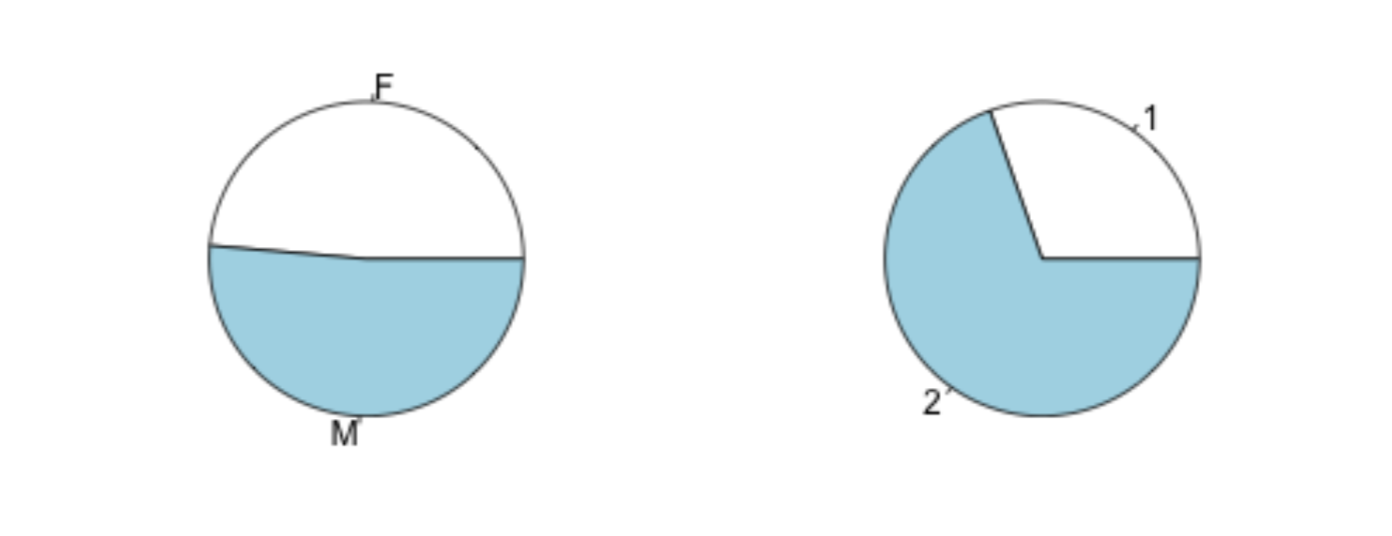
\includegraphics[width=0.7\linewidth]{wolf_sex.png}
		\caption{kjønnsfordelingen blandt ulvepopulasjonen er svært jevnt fordelt, hvilket nesten alltid er tilfellet pga naturlig seleksjon. Omtrent to tredeler er tungt jaktet}
		\label{fig:sex_population}
\end{figure}

\subsection*{c}

Denne oppgaven løser jeg ved å bruke kommandoene \texttt{wolf.lett <- wolf[wolf[,"population"]==1,]} og \texttt{wolf.tungt <- wolf[wolf[,"population"]==2,]}, slik jeg ble fortalt i oppgaven.

\subsection*{d}

\begin{figure}[H]
		\centering
		\includegraphics[width=0.7\linewidth]{wolf_sammenlign.pdf}
		\caption{a) Formen på histogramet minner om normalfordeling, men med litt for mange verdier høyt oppe. b) Formen minner mindre på en normalfordeling, men vi legger merke til at stolpene er tykkere enn for a) og at det ikke er like mange høye verdier. Forskjellen i verdier er høyere for lett enn tungt.}
		\label{fig:sammenlign}
\end{figure}

\subsection*{e}

\begin{center}
\label{tab:mean_median_standard}
\captionof{table}{Vi ser det jeg sa i forrige oppgave. SD er mindre for tungt enn for lett. Gjennomsnittet er lavere for lett, men dette gjør at du for et høyere standardavvik (pga de høye verdiene vi så i figur \ref{fig:sammenlign} a))}
\begin{tabularx}{\textwidth}{c X c X c X c }
    \hline
    \hline
         && Mean && Median && Standard deviation \\
    \hline
    \\
        Lett   	&&     15.56222      &&      14.24      &&     7.298785       \\
        Tungt   &&     17.07495      &&      16.32      &&      5.543389       \\
    \hline
\end{tabularx}
\end{center}


\subsection*{f}

FEMTALLS: min,Q$_1$,$\mu$,Q$_3$,max
\\
Gjennomsnitt og standardavvik: $\mu \land \sigma$
\\
\\
Vel, er ikke dette dumt å spørre om før vi har gjort g? Hvis dataen ligner på en normalfordeling burde en bruke gjennomsnitt og standardavvik. Hvis det er en jevn fordeling, så er det bedre med femtallsoppsummering. 

\subsection*{g}

\begin{figure}[H]
    \centering
    \begin{subfigure}{0.5\textwidth}
        \centering
        \includegraphics[width=\linewidth]{LETT.pdf}
        \caption{}
    \end{subfigure}%
    ~
    \begin{subfigure}{0.5\textwidth}
        \centering
        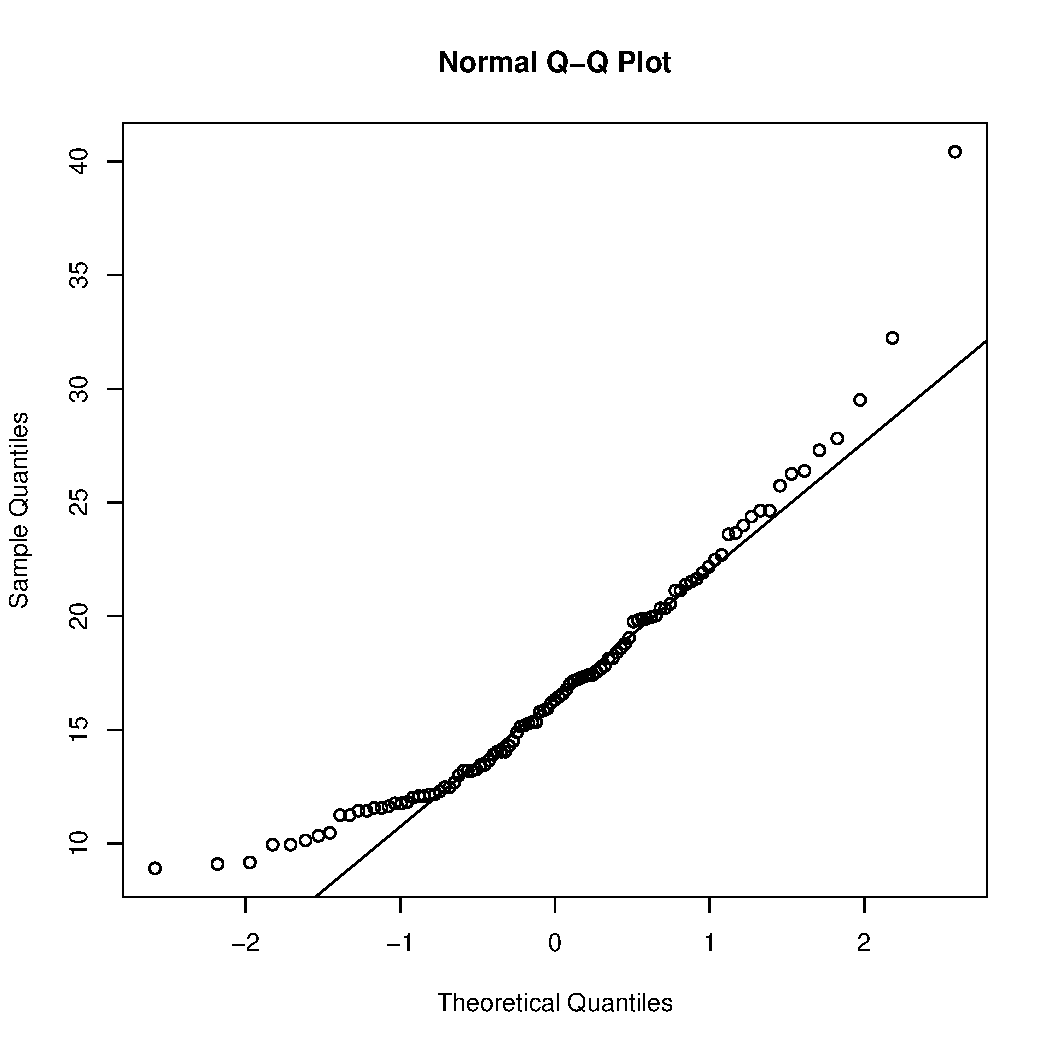
\includegraphics[width=\linewidth]{TUNGT.pdf}
        \caption{}
    \end{subfigure}
    \caption{a) Datapunktene ser jevnt fordelt ut over x-verdien. Datapunktene ligger ikke spesielt bra på linjen. b) Datapunktene ser ikke jevnt fordelt ut over x-verdien. Det er en større andel som ligger mot x = 0. Majoriteten til datapunktene ligger bra på linjen. }
    \label{fig:2G}
\end{figure}

Fra figur \ref{fig:2G} ser det ut til at tungt er normalfordelt. Lett ser ikke ut til å være det. Ergo; femtallsoppsummering for lett og gjennomsnitt og standardavvik for tungt. 






























\pagebreak
\section{}

\subsection*{a}

150 kvinner og 73 menn deltok i forsøket! 

\begin{center}
\label{tab:summary}
\captionof{table}{Tabellen viser en oversikt over femtallsoppsummeringen til de fire målingene i datasettet.}
\begin{tabularx}{\textwidth}{c X c X c X c X c X c }
    \hline
    \hline
         && min && $Q_1$ && $\mu$ && $Q_3$ && max \\
    \hline
    kroppslengde   	&& 152.0 && 166.0 && 172.3 && 178.0 && 196.0 \\
    fot.navle    	&&  87.0 && 101.0 && 104.8 && 109.0 && 125.0 \\
    navle.isse	 	&& 52.00 && 65.00 && 67.34 && 70.00 && 81.00 \\
    favn			&& 146.0 && 165.0 && 172.4 && 180.0 && 202.0 \\

    \hline
\end{tabularx}
\end{center}

\subsection*{b}

\begin{figure}[H]
		\centering
		\includegraphics[width=0.4\linewidth]{3B.pdf}
		\caption{Figuren viser kroppshøyde som funksjon av navlelengde. En skulle nesten tro at det var en høy korrelasjon mellom disse to variablene.}
		\label{fig:3B}
\end{figure}



\subsection*{c}
Ooooo, ser man det! Det var en høy korrelasjon mellom de.
cor funksjonen gir 0.9140397. Det vil si at høyden til et menneske er høyt avhengig av høyden til navlen for det mennesket. 

\subsection*{d}
Jeg tok meg friheten til å skifte på koden gitt i obligen, slik at programmet mitt kjørte. 


\begin{figure}[H]
		\centering
		\includegraphics[width=0.7\linewidth]{3D.pdf}
		\caption{Dette ser jo bra ut. }
		\label{fig:3D}
\end{figure}


\subsection*{e}
Summary funket dårlig. Jeg brukte print(fit) for å fastslå koeffisientene til modellen. Hvis navlehøyden øker med en cm øker høyden med 1.273 cm.

\begin{center}
\label{tab:e}
\captionof{table}{Coefficients for the linear model}
\begin{tabularx}{\textwidth}{c X c X c }
    \hline
    \hline
        Coefficients && a && b\\
    \hline
				   	&& 38.897 && 1.273\\
    \hline
\end{tabularx}
\end{center}

\subsection*{f}
Kroppshøyden til en person med navlehøyde på 121 cm vil med modellen min bli predikert til 192.93 cm. 

\begin{align*}
	f(121)= a + b*x = 192.93
\end{align*}

\pagebreak
\subsection*{g}

\begin{center}
\label{tab:summary2}
\captionof{table}{...}
\begin{tabularx}{\textwidth}{c X c X c X c X c X c }
    \hline
    \hline
         && min && $Q_1$ && $\mu$ && $Q_3$ && max \\
    \hline
    kroppslengde   	&& 152.0 && 166.0 && 172.3 && 178.0 && 196.0 \\
    fot.navle    	&&  87.0 && 101.0 && 104.8 && 109.0 && 125.0 \\
    navle.isse	 	&& 52.00 && 65.00 && 67.34 && 70.00 && 81.00 \\
    favn			&& 146.0 && 165.0 && 172.4 && 180.0 && 202.0 \\

    \hline
\end{tabularx}
\end{center}


\subsection*{h}

\begin{figure}[H]
		\centering
		\includegraphics[width=0.7\linewidth]{3H.pdf}
		\caption{...}
		\label{fig:3H}
\end{figure}


































\pagebreak

\section*{Appendix}


\begin{lstlisting}[language=python]

#OPPGAVE 1
from matplotlib.pyplot import *			#import av shit
from numpy import *			#import av shit
import scipy.integrate as integrate		#import av shit

infile = open("data.txt","r")			#aapne fil
infile.readline()				#aapne fil

x = []				#tomme lister
hist_list = []			#tomme lister
for line in infile.readlines():		#leser fil
	words = line.split(" ")			#leser fil
	hist_list.append(float(words[1]))	#leser fil
	x.append(int(eval(words[0])))		#leser fil

s = std(hist_list) 	#standard deviation
m = mean(hist_list) #gjennomsnitt

def gaussian(x,s=s,m=m):#gaussian funksjon
	return (1/(sqrt(2*pi)*s))*exp(-0.5*((x-m)/s)**2) #formelen for gaussianfordeling

def integral(fra=0,til=100,func = gaussian): #funksjon
	return integrate.quad(func,fra,til)[0]	#numpy sin integrate funksjon

if __name__ == '__main__':
	print(integral(0,0.6))	#INTEGRAL
	print(integral(1,100))	#INTEGRAL
	print(integral(0,100))	#INTEGRAL
\end{lstlisting}








\pagebreak
\begin{lstlisting}[language=R]
#OPPGAVE 1
# data = "http://www.uio.no/studier/emner/matnat/math/STK1000/data/zebrafinch.txt"
# zebrafinch <- read.table(data,header=TRUE)

# Create data for the graph.
zebrafinch <- c(0.7562718,0.7841234,0.8535867,0.82394,0.7804905,0.9630961,0.7417845,1.120064,0.8024751,0.8214675,0.7309519,0.8019651,0.9097601,0.7601681,0.8390591,0.9248859,0.8352816,0.7319939,0.7930914,0.7457873,1.002192,0.8628477,1.028025,0.7402723,0.9129746,0.7300062,0.8572898,0.8500707,0.7334023,0.7144842,0.984181,0.8167179,0.8441634,0.8281507,0.6719701,0.8034057,1.11701,1.007286,0.8168411,0.7305809,0.9279448,0.8405102,0.7958567,0.9990197,1.007542,0.6806091,0.8384404,0.8711419,0.7179686,0.9287494,0.8619765,0.8309871,0.5787197,0.7416669,0.8040855,0.8081294,0.907542,0.8482643,0.8560268,0.8655504,1.172754,0.9761892,0.8843472,0.9139844,0.5186183,0.9385081,0.9074842,0.9329575,1.090915,0.7363603,0.8898355,0.8577158,1.025406,0.6654378,0.6658608,0.6768501,0.9794527,0.8301966,0.8290008,0.8836586,0.8157841,0.964259,0.9287292,0.9011676,0.7669517,0.7306965,0.9245895,0.9635717,0.7862857,0.8990346,0.7850173,0.8521878,0.7135978,0.8522143,0.8528686,0.9675156,0.6637724,0.8162315,0.9481493,0.867313,0.936353,0.986539,0.8309639,0.7233021,1.044636,0.6885234,0.9870739,0.7755702,0.7006348,0.8671587,1.109845,0.9798947,0.8143468,0.8347534,0.8840403,0.7789924,0.7760159,0.8019032,0.6420586,0.8729059,0.8722336,0.7732556,0.9370564,0.8527847,0.9538383,0.8060772,0.7286053,0.8899104,0.7440977,0.9768809,1.050496,0.5891953,0.8203677,0.8185292,0.7594463,0.8304673,0.9525384,0.966009,0.8968909,0.9481618,0.738298,0.7978259,0.7972277,0.6588164,0.9295452,1.002859,0.9822667,0.8677425,0.8259351,0.8138577)

#sum(zebrafinch/150)
mean(zebrafinch)			#AVERAGE = 0.8485003
sd(zebrafinch)				#Standard deviation
IQR(zebrafinch)				#Interquartile
median(zebrafinch)			#MEDIAN

# Standardiserte verdien til 0.8 er lik:
print((0.8-mean(zebrafinch))/sd(zebrafinch))
#-0.4276918 standardavvik til normalfordelingen


# Give the chart file a name.
png(file = "zebrafish.pdf")
# Create the histogram.
hist(zebrafinch,xlab = "Weight",col = "yellow",border = "blue")

# Save the file.
dev.off()


qqnorm(zebrafinch) #lager qq plot
qqline(zebrafinch) #lager qq plot
# pnorm(zebrafinch) #NEI TAKK
\end{lstlisting}



\pagebreak
\begin{lstlisting}[language=R]
#OPPGAVE 2222222222222222222222222222222222222222

#AAAAAAAAAAAAAAAAAAAAAAAAAAAAAAAAAAAAAAAAAAAAAAAA
data ="http://www.uio.no/studier/emner/matnat/math/STK1000/data/wolves.txt"
wolf <- read.table(data,header=TRUE)
# print(c(wolf))
# print(wolf$sex)
# print(wolf$population)
# print(wolf$tpmg)
# print(wolf$cpmg)

#BBBBBBBBBBBBBBBBBBBBBBBBBBBBBBBBBBBBBBBBBBBBBBBB
# Give the chart file a name.
png(file = "wolf_sex.png")
par(mfrow=c(1,2)) #MAKING TWO COLUMNS
pie(table(wolf$sex))# Create the histogram.
pie(table(wolf$population))# Create the histogram.
dev.off()# Save the file.

#CCCCCCCCCCCCCCCCCCCCCCCCCCCCCCCCCCCCCCCCCCCCCCCC
#NOT MY IDEA!
wolf.lett <- wolf[wolf[,"population"]==1,]
wolf.tungt <- wolf[wolf[,"population"]==2,]

#DDDDDDDDDDDDDDDDDDDDDDDDDDDDDDDDDDDDDDDDDDDDDDDD
png(file = "wolf_sammenlign.png")		#was told this
par(mfrow=c(2,2))			#was told this
hist(wolf.lett$cpmg)				#was told this
boxplot(wolf.lett$cpmg)				#was told this
hist(wolf.tungt$cpmg)				#was told this
boxplot(wolf.tungt$cpmg)			#was told this
dev.off()				#was told this

#EEEEEEEEEEEEEEEEEEEEEEEEEEEEEEEEEEEEEEEEEEEEEEEE
mean(wolf.lett$cpmg)		#average
median(wolf.lett$cpmg)		#median
sd(wolf.lett$cpmg)			#Standard deviation
mean(wolf.tungt$cpmg)		#average
median(wolf.tungt$cpmg)		#median
sd(wolf.tungt$cpmg)			#Standard deviation

#FFFFFFFFFFFFFFFFFFFFFFFFFFFFFFFFFFFFFFFFFFFFFFFF
#EHM tekst... 

#GGGGGGGGGGGGGGGGGGGGGGGGGGGGGGGGGGGGGGGGGGGGGGGG
qqnorm(wolf.tungt$cpmg)		#QQ plot
qqline(wolf.tungt$cpmg)		#QQ plot
qqnorm(wolf.lett$cpmg)		#QQ plot
qqline(wolf.lett$cpmg)		#QQ plot
\end{lstlisting}





















\pagebreak
\begin{lstlisting}[language=R]
#OPPGAVE 333333333333333333333333333

data = "http://www.uio.no/studier/emner/matnat/math/STK1000/data/vitruvisk.txt"
vitruvisk <- read.table(data,header=TRUE)

#AAAAAAAAAAAAAAAAAAAAAAAAAAAAAAAAAAA
summary(vitruvisk)

#BBBBBBBBBBBBBBBBBBBBBBBBBBBBBBBBBBB
# Give the chart file a name.
png(file = "3B.pdf")
plot(vitruvisk$fot.navle,vitruvisk$kroppslengde,xlab="navlehoyde",
ylab="kroppslengde")
# Save the file.
dev.off()

#CCCCCCCCCCCCCCCCCCCCCCCCCCCCCCCCCCC
cor(vitruvisk$fot.navle,vitruvisk$kroppslengde)

#DDDDDDDDDDDDDDDDDDDDDDDDDDDDDDDDDDD
# Give the chart file a name.
png(file = "3D.pdf")
plot(vitruvisk$fot.navle,vitruvisk$kroppslengde,xlab="navlehoyde",
ylab="kroppslengde")
fit <- lm(kroppslengde ~ fot.navle,data =  vitruvisk)
abline(fit)

# Save the file.
dev.off()

#EEEEEEEEEEEEEEEEEEEEEEEEEEEEEEEEEEE
summary(fit)
print(fit)

#FFFFFFFFFFFFFFFFFFFFFFFFFFFFFFFFFFF
print(38.897 + 121*1.273)

#GGGGGGGGGGGGGGGGGGGGGGGGGGGGGGGGGGG
summary(vitruvisk)

#HHHHHHHHHHHHHHHHHHHHHHHHHHHHHHHHHHH
png(file = "3H.pdf")
plot(vitruvisk$fot.navle,residuals(fit))
abline(h=0)
# Save the file.
dev.off()
\end{lstlisting}






















%\begin{align*}
%&n \qquad &2^n - (-1)^n\\
%&n+1 \qquad &2^{n+1} - (-1)^{n+1} \\
%& &= 2(2^{n}) - (-1)^{n+1}\\
%& &= 2(2^{n} + (-1)^n  + (-1)^{n+1}) - (-1)^{n+1}\\
%& &= 2(2^{n} + (-1)^n  - (-1)^{n}) - (-1)^{n+1}\\
%& &= 2(2^{n}- (-1)^{n}) + 2(-1)^n  + (-1)^{n}\\
%& &= 2(2^{n}- (-1)^{n}) + 3(-1)^n \\
%\end{align*}



% \begin{figure}[H]
%     \centering
%     \begin{subfigure}{0.5\textwidth}
%         \centering
%         \includegraphics[width=\linewidth]{result/bilder/Tc/e-Tc}
%         \caption{}
%     \end{subfigure}%
%     ~
%     \begin{subfigure}{0.5\textwidth}
%         \centering
%         \includegraphics[width=\linewidth]{result/bilder/Tc/m-Tc}
%         \caption{}
%     \end{subfigure}
%     \caption{a) Shows how E behaves around $T_C$ b) Shows how |M| develops near $T_C$.}
%     \label{fig:tc-E-M}
% \end{figure}






% \begin{center}
% \label{tab:states-2x2-summary}
% \captionof{table}{The table shows a summary from table \ref{tab:states-2x2}. }
% \begin{tabularx}{\textwidth}{c X c X c X c}
%     \hline
%     \hline
%         Number of $\color{red}{\uparrow}$ && Multiplicity && Energy && Magnetic moment \\
%     \hline
%         4   &&      1      &&      -8J     &&       4       \\
%         3   &&      4      &&      0J      &&       2       \\
%         2   &&      2      &&      8J      &&       0       \\
%         2   &&      4      &&      0J      &&       0       \\
%         1   &&      4      &&      0J      &&       -2      \\
%         0   &&      1      &&      -8J     &&       -4      \\
%     \hline
% \end{tabularx}
% \end{center}













%\begin{tabular}{|c|c|c|c|c|c|c|}
%	\hline
%	n & General & Specific & LU & fastest & slowest & $\frac{slowest}{fastest}$\\
%	\hline
%	10 & 6.5e-05 & 5e-06 & 4e-05 & Specific & General & 13.0\\
%	\hline
%	100 & 7.5e-05 & 8e-06 & 0.0023 & Specific & LU & 287.5\\
%	\hline
%	1000 & 0.00014 & 4e-05 & 0.26 & Specific & LU & 6500\\
%	\hline
%	10000 & 0.0007 & 0.0005 & 142.5 & Specific & LU & 285000 \\
%	\hline
%\end{tabular}







%\begin{figure}[H]
%		\centering
%		\includegraphics[width=0.7\linewidth]{ab.png}
%		\caption{Atomene er gule kuler, de elementære vektorene er blå og a vektorene er grønne.}
%		\label{fig:ab}
%\end{figure}



%\begin{figure}[H]
%		\centering
%		\includegraphics[width=0.7\linewidth]{ab.png}
%		\caption{Atomene er gule kuler, de elementære vektorene er blå og a vektorene er grønne.}
%		\label{fig:ab}
%\end{figure}
%\printbibliography






%\begin{figure}[H]
%    \centering
%    \begin{subfigure}{0.5\textwidth}
%        \centering
%        \includegraphics[width=\linewidth]{maybe}
%        \caption{}
%    \end{subfigure}%
%    ~
%    \begin{subfigure}{0.5\textwidth}
%        \centering
%        \includegraphics[width=\linewidth]{maybe2}
%        \caption{}
%    \end{subfigure}%
%    \caption{a) is probably wrong and b) is right? If not i am not sure what to comment. No matter what. I am not sure what to comment. Cause b) should be wrong. The code above produces a). Setting kb to 1 gives b)}
%\end{figure}








%\begin{align*}
%	J (x,y)=
%	\begin{bmatrix}
%		12x^2 & 1\\
%		1 & 2
%	\end{bmatrix}
%\end{align*}



\end{document}
